\documentclass{article}

\usepackage{amsfonts}
\usepackage{graphicx}
\usepackage{stmaryrd}
\usepackage{nccmath}
\usepackage[french]{babel}
\selectlanguage{french} 
\newcommand{\A}[0]{{\cal A}}
\newcommand{\C}[0]{{\cal C}}
\newcommand{\se}[1]{\medbreak \medbreak \section*{#1}}
\newcommand{\sse}[1]{\medbreak \subsection*{#1}}
\newcommand{\ssse}[1]{\subsubsection*{#1}}
\newcommand{\Def}[0]{\ssse{D�finition}}
\newcommand{\The}[0]{\ssse{Th�or�me}}
\newcommand{\Pro}[0]{\ssse{Propri�t�}}
\newcommand{\mb}[1]{\mathbb{#1}}
\newcommand{\Exo}[1]{\sse{Exercice #1}}
\newcommand{\Que}[1]{\ssse{Question #1}}
\newcommand{\ssi}[0]{\leftrightarrow}
\newcommand{\ra}[0]{\rightarrow}
\newcommand{\Ra}[0]{\Rightarrow}
\newcommand{\la}[0]{\leftarrow}
\newcommand{\La}[0]{\Leftarrow}
\newcommand{\llb}[0]{\llbracket}
\newcommand{\rrb}[0]{\rrbracket}
\newcommand{\dd}[0]{\txt{d}}
\newcommand{\dr}[0]{\partial}
\newcommand{\txt}[1]{\textrm{#1}}
\newcommand{\ol}[1]{\overline{#1}}
\newcommand{\ul}[1]{\underline{#1}}
\newcommand{\abs}[1]{|#1|}
\newcommand{\iso}[0]{\simeq}
\usepackage[french,onelanguage]{algorithm2e}

\usepackage{graphicx}
\usepackage[utf8]{inputenc}  
\usepackage[T1]{fontenc}    

\begin{document}
\sse{Pseudo code : périodisation "inclinée"}
On suppose que l'on reçoit l'image initiale transformée par affinité (cf figure : \ref{affinit}), et donc plongée dans une image plus grande (on complète l'image par la moyenne de l'image de départ (l'image de tout départ étant le dragon et le blanc, sans tout le gris autour et droite). \\
Le fonction du code est de prendre deux point de coordonnée quelconque et de les ramener dans l'image blanche avec le dragon (ce qui permet de périodiser l'image en fait).\\

\begin{figure}
\begin{center}
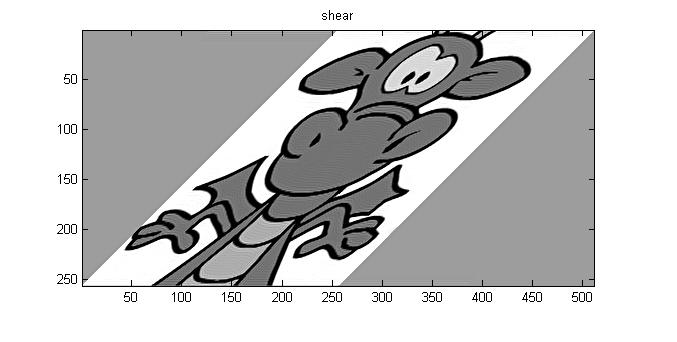
\includegraphics[width=75mm]{shear.jpg}
\end{center}
\caption{Image après affinité (on veut périodiser le dragon et le blanc au milieu)}
\label{affinit}
\end{figure}


\begin{figure}
\begin{center}
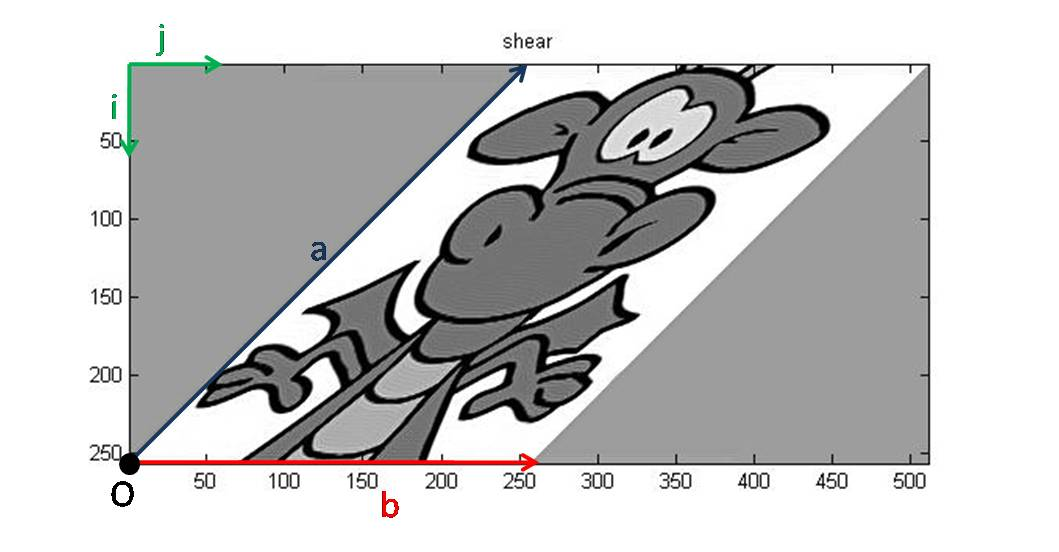
\includegraphics[width=75mm]{shearexp.jpg}
\end{center}
\caption{base : explication}
\label{affinite}
\end{figure}


On suppose que les vecteurs "a" et "b" sont comme défini sur la figure \ref{affinite} s'exprimment dans la base (i,j) (aussi définie sur la même figure) de la façon suivante : \\
$a=a(1)*j+a(2)*i$ et \\
$b=b(1)*j+b(2)*i$ \\

J'ai testé le code pour i et j de norme 1 (1 pixel) et a et b de norme la la longeur en pixel de chaque côté de l'image après le shear (ils sont représenté à l'échelle sur la figure \ref{affinite}, contrairement à i et j). "O" est l'origine de la nouvelle base (comme indiqué sur la figure).

\begin{algorithm}
\caption{Périodisation}
\KwData{les vecteurs a et b et O (O est le centre de la nouvelle base) exprimmés dans la base (i,j), le couple de points (ui,uj) de départ de coordonnées réelles dans (i,j)}
En sortie : Le couple de points (vi,vj) (de coordonées réelles dans (i,j)).  \;
Notations : \\
a=(a1,a2)\\
b=(b1,b2)\\
O=(oi,oj)\\
Changement d'origine :\\
 wi=ui-oi ;\\
wj=uj-oj ;\\
Changement de base :\\
det=a1*b2-b1*a2 ;\\
wa=(b2*wj-b1*wi)/det ;\\
wb=(-a2*wj+a1*wi)/det ;\\

réduction modulo les vecteurs (a et b) (ici dans la novelle base (O,a,b), ils sont de norme 1,
donc on prend la partie non-entière).\\

ra=wa-floor(wa) ;\\
rb=wb-floor(wb) ;\\

  changement de base inverse :\\

wi=ra*a2+rb*b2 ;\\
wj=ra*a1+rb*b1 ;\\

 retour à l'origine :\\
 
vi=wi+oi ;\\
vj=wj+oj ;\\


\KwRet{(vi,vj)}
\end{algorithm}

Attention : à la fin on a deux points réels à priori. On peut ensuite en prendre la partie entière des points pour se ramener à des entiers.\\
Remarque : On peut utiliser cette technique pour effectuer un mipmap après un shear. Il suffit de construire un mipmap avec l'image après le shear (par exemple un mipmap à une dimension comme en figure \ref{mipmap}). Il suffit ensuite de lors de la lecture du mip-map d'utiliser le programme décrit plus haut en n'oubliant pas de diviser les coordonnées des vecteurs a et b par la puissance de 2 qui convient (cette puissance de 2 étant différente pour a et pour b dans le cas du ripmap) . On a le résultat d'un tel procédé figure \ref{trans}.\\
Remarque 2 : La technique n'est pas parfaite à 1 pixel près : Sur les bords de l'image il y a toujours le risque de tomber sur un pixel que l'on ne veut pas lorsque l'on prend la partie entière (cf figure \ref{def}). En pratique si on travail sur des images périodisée, on ne voit pas de problème.

\begin{figure}
\begin{center}
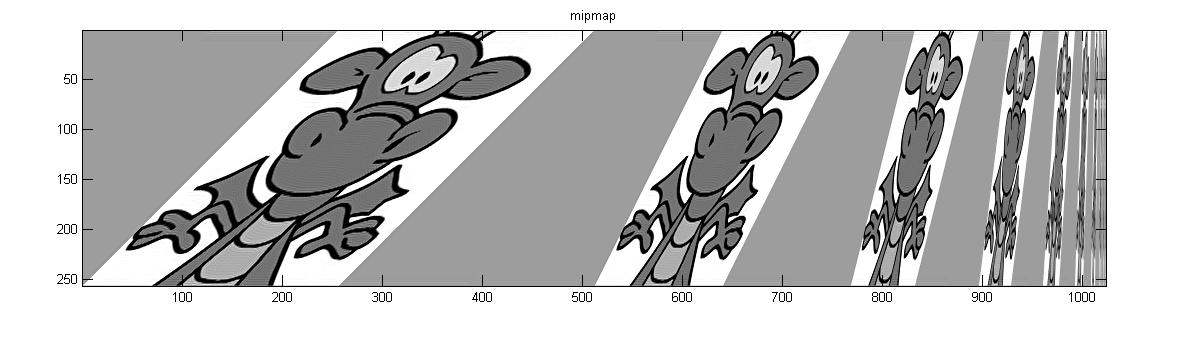
\includegraphics[width=75mm]{mipmap1d.jpg}
\end{center}
\caption{Mipmap une dimension}
\label{mipmap}
\end{figure}


\begin{figure}
\begin{center}
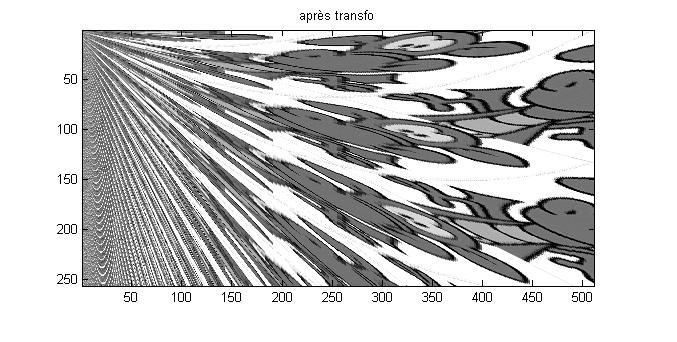
\includegraphics[width=75mm]{result.jpg}
\end{center}
\caption{transformation par mipmap une dimension}
\label{trans}
\end{figure}

\begin{figure}
\begin{center}
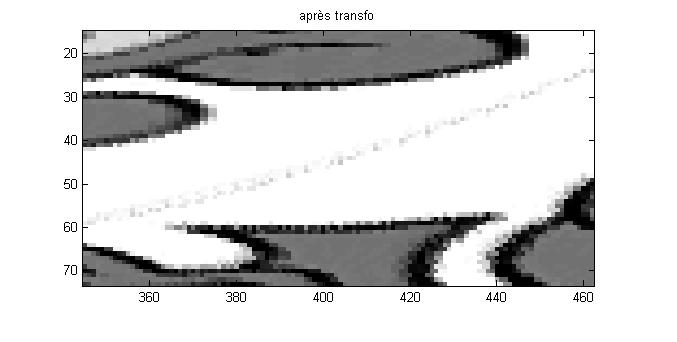
\includegraphics[width=75mm]{default.jpg}
\end{center}
\caption{défaut}
\label{def}
\end{figure}

\end{document}